\documentclass[a4paper,12pt]{article}
\usepackage[utf8]{inputenc}
\usepackage[spanish]{babel}
\usepackage{color}
\usepackage{parskip}
\usepackage{graphicx}
\usepackage{multirow}
\usepackage{listings}
\usepackage{vmargin}
\graphicspath{ {imagenes/} }
\definecolor{mygreen}{rgb}{0,0.6,0}
\definecolor{lbcolor}{rgb}{0.9,0.9,0.9}
\usepackage{epstopdf}


\setpapersize{A4}
\setmargins{2.5cm}       % margen izquierdo
{1.5cm}                        % margen superior
{16.5cm}                      % anchura del texto
{23.42cm}                    % altura del texto
{10pt}                           % altura de los encabezados
{1cm}                           % espacio entre el texto y los encabezados
{0pt}                             % altura del pie de página
{2cm}     

\lstset{
backgroundcolor=\color{lbcolor},
    tabsize=4,    
%   rulecolor=,
    language=[GNU]C++,
        basicstyle=\tiny,
        aboveskip={1.5\baselineskip},
        columns=fixed,
        showstringspaces=false,
        extendedchars=false,
        breaklines=true,
        prebreak = \raisebox{0ex}[0ex][0ex]{\ensuremath{\hookleftarrow}},
        frame=single,
        showtabs=false,
        showspaces=false,
        showstringspaces=false,
        identifierstyle=\ttfamily,
        keywordstyle=\color[rgb]{0,0,1},
        commentstyle=\color[rgb]{0.026,0.112,0.095},
        stringstyle=\color{red},
        numberstyle=\color[rgb]{0.205, 0.142, 0.73},
%        \lstdefinestyle{C++}{language=C++,style=numbers}’.
}

\begin{document}

\begin{Large}
 NOMBRE: CHRISTOFER FABIÁN CHÁVEZ CARAZAS
\end{Large}

\section{Problema}

Resolver las partes ``a'' y ``b'' del problema 2.2.23.

\section{Resolución}

El programa creado está diseñado para resolver los dos problemas. Se necesita ingresar un número $x$ con el
cual se generará la matriz X. Las matrices de error se generan con un número $n$ muy pequeño.
En nuestro caso $x=10$ y $n=0.0000001$.

\begin{lstlisting}
#include <iostream>
#include "OperacionesMatriz.h"

using namespace std;

int main(){
	Num n = 0.0000001;
	int tipo;
	Num x;
	cout<<"Que problema quiere resolver: b (1) - c (2) ->";
	cin>>tipo;
	cout<<"Con que x quieres trabajar ->";
	cin>>x;
	Matriz A = {{375,374},{752,750}};
	Lista X = createLista(x,A.size());
	Lista alfa = createLista(n,A.size());
	Lista b = A * X;
	cout.precision(20);
	if(tipo == 1){
		cout<<"----X----"<<endl;
		mostrarLista(alfa);
		cout<<"----aX----"<<endl;
		X = X - alfa;
		mostrarLista(X);
		cout<<"----error----"<<endl;
		cout<<normInf(X) / normInf(alfa)<<endl;

		cout<<"----B----"<<endl;
		b = b - alfa;
		mostrarLista(b);
		cout<<"----aB----"<<endl;
		mostrarLista(alfa);
		cout<<"----error----"<<endl;
		cout<<normInf(alfa) / normInf(b)<<endl;
	}
	else if(tipo == 2){
		cout<<"----X----"<<endl;
		X = X - alfa;
		mostrarLista(X);
		cout<<"----aX----"<<endl;
		mostrarLista(alfa);
		cout<<"----error----"<<endl;
		cout<<normInf(alfa) / normInf(X)<<endl;

		cout<<"----B----"<<endl;
		mostrarLista(alfa);
		cout<<"----aB----"<<endl;
		b = b - alfa;
		mostrarLista(b);
		cout<<"----error----"<<endl;
		cout<<normInf(b) / normInf(alfa)<<endl;	
	}
}
\end{lstlisting}

\subsection{Resultado a)}

\vspace{5mm}

\begin{figure}[h]
\centering
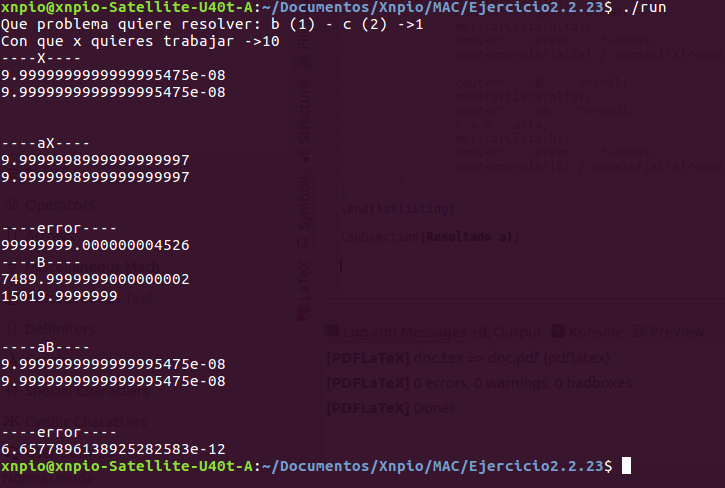
\includegraphics[scale=0.5]{1.png}
\end{figure}

\subsection{Resultado b)}

\begin{figure}[h]
\centering
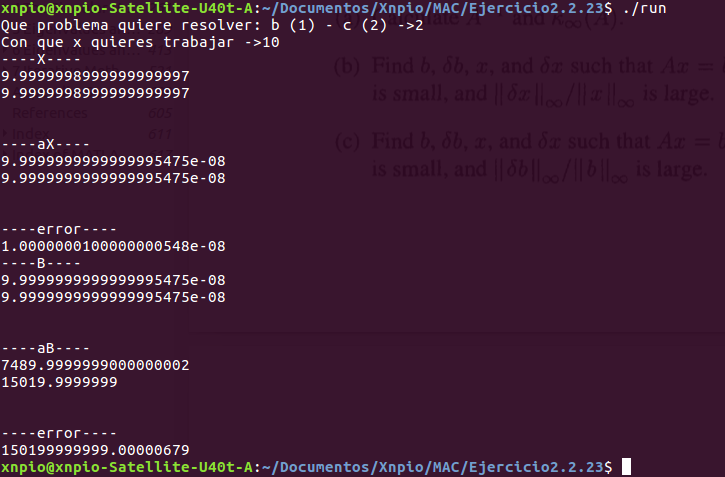
\includegraphics[scale=0.5]{2.png}
\end{figure}


\end{document}
